
\noindent\rule{7in}{2.8pt}
\section{Electron-Proton Elastic Scattering}
    
\begin{problem}{7.1}
The derivation of (7.8) used the algebraic relation

\begin{align*}
    \left(\gamma+1\right)^2 \left(1-\kappa^2\right)^2 = 4,
\end{align*}\\
where 

\begin{align*}
    \kappa = \frac{\beta\gamma}{\gamma+1} \andtxt \left(1-\beta^2\right)\gamma^2 = 1
\end{align*}\\
Show that this holds.
\end{problem}
\begin{solution}
Using the given relation of $\kappa$ in terms of $\beta,\gamma$,

\begin{align*}
    (\gamma+1)^2 (1-\kappa^2)^2 &= (\gamma+1)^2 \left[ 1- \frac{\beta^2\gamma^2}{(\gamma+1)^2} \right]^2 \\[0.12in]
                                &= \left[ (\gamma+1) - \frac{\beta^2\gamma^2}{\gamma+1} \right]^2 \impliedby \beta^2\gamma^2 = \gamma^2 - 1 \\[0.12in]
                                &= \left[ (\gamma+1) - \frac{\gamma^2-1}{\gamma+1} \right]^2 = \left[ (\gamma+1) - (\gamma-1) \right]^2 = 4 \qed
\end{align*}
\end{solution}

\noindent\rule{7in}{1.5pt}

%%%%%%%%%%%%%%%%%%%%%%%%%%%%%%%%%%%%%%%%%%%%%%%%%%%%%%%%%%%%%%%%%%%%%%%%%%%%%%%%%%%%%%%%%%%%%%%%%%%%%%%%%%%%%%%%%%%%%%%%%%%%%%%%%%%%%%%%

\begin{problem}{7.2}
    By considering momentum and energy conservation in $e^-p$ elastic scattering from a proton at rest, find an expression for the fractional energy loss of the scattered electron $\left( E_1 - E_3 \right)/E_1$ in terms of the scattering angle and the parameter

    \begin{align*}
        \kappa = \frac{p}{E_1 +m_e} \equiv \frac{\beta\gamma}{\gamma+1}
    \end{align*}
\end{problem}
\begin{solution}
The author stated in the \href{https://www.hep.phy.cam.ac.uk/~thomson/MPP/ModernParticlePhysics_Errata.pdf}{\texttt{errata}} that this problem should be ignored. 
\end{solution}

\noindent\rule{7in}{1.5pt}

%%%%%%%%%%%%%%%%%%%%%%%%%%%%%%%%%%%%%%%%%%%%%%%%%%%%%%%%%%%%%%%%%%%%%%%%%%%%%%%%%%%%%%%%%%%%%%%%%%%%%%%%%%%%%%%%%%%%%%%%%%%%%%%%%%%%%%%%

\begin{problem}{7.3}
    In an $e^-p$ scattering experiment, the incident electron has energy $E_1 = 529.5 \MeV$ and the scattered electrons are detected at an angle of $\theta = 75^\circ$ relative to the incoming beam.
    \begin{enumerate}[label=(\alph*)]
        \item At this angle, almost all of the scattered electrons are measured to have an energy of $E_3 \approx 373 \MeV$. What can be concluded from this observation?
        \item Find the corresponding value of $Q^2$.
    \end{enumerate}
\end{problem}
\begin{solution}
\begin{enumerate}[label=(\alph*)]
    \item Let us assume that these observed electrons experienced a relativistic elastic scattering with the proton, then under such hypothesis the measured electron energy after the scattering process $E_3$ shall be :
    
    \begin{align*}
        E_3 = \frac{E_1 m_p}{m_p + E_1 (1-\cos\theta)} \simeq \frac{530\MeV \cdot 940 \MeV}{940 \MeV + 530 \MeV \cdot (1-0.25)} \simeq 372 \MeV
    \end{align*}\\
    which well corresponds with most of the observed energy of the scattered electrons. This implies that these electrons actually underwent an elastic collision with the proton, and the proton in concern remains intact.

    \item Using the observed values, 
    
    \begin{align*}
        Q^2 = \frac{2m_p E_1^2(1-\cos\theta)}{m_p + E_1 (1-\cos\theta)} \simeq \frac{2\cdot 940 \MeV \cdot 530^2 \MeV^2 \cdot (1-0.25)}{940 \MeV + 530 \MeV \cdot (1-0.25)} \simeq \boxed{0.32 \GeV^2}
    \end{align*}
\end{enumerate}
\end{solution}

\noindent\rule{7in}{1.5pt}

%%%%%%%%%%%%%%%%%%%%%%%%%%%%%%%%%%%%%%%%%%%%%%%%%%%%%%%%%%%%%%%%%%%%%%%%%%%%%%%%%%%%%%%%%%%%%%%%%%%%%%%%%%%%%%%%%%%%%%%%%%%%%%%%%%%%%%%%

\begin{problem}{7.4} \customlabel{P7.4}{7.4}
    For a spherically symmetric charge distribution $\rho(r)$, where

    \begin{align*}
        \int \rho(r) \dif^3 \mathbf{r} = 1,
    \end{align*}\\
    show that the form factor can be expressed as

    \begin{align*}
        F(\mathbf{q}^2) = \frac{4\pi}{q} \int^\infty_0 r \sin(qr) \rho(r) \dif r \simeq 1 -\frac{1}{6}q^2\expval{R^2} + \cdots
    \end{align*}\\
    where $\expval{R^2}$  is the mean square charge radius. Hence show that,

    \begin{align*}
        \expval{R^2} = -6 \left[ \frac{\dif F(\mathbf{q}^2)}{\dif q^2} \right]_{q^2=0}
    \end{align*}
\end{problem}
\begin{solution}
Starting from the definition of the form factor, and letting $\theta$ be the angle between $\mathbf{q}$ and $\mathbf{r}$ while $\phi$ as the azimuthal angle, 

\begin{align*}
    F(q^2) &= \int \rho(r) \exp\left[i\mathbf{q}\cdot\mathbf{r}\right] \dif^3 \mathbf{r} \\[0.12in]
           &= -\int \rho(r) \exp\left[ iqr\cos\theta \right]  r^2 \dif r \dif \cos\theta \dif \phi \\[0.12in]
           &=  2\pi \int_0^\infty r^2 \rho(r) \int_{-1}^{+1} \exp\left[ iqr\cos\theta \right] \dif \cos\theta    \dif r \\[0.12in]
           &= 2\pi \int_0^\infty r^2 \rho(r) \frac{2}{qr} \sin(qr) \dif r = \frac{4\pi}{q} \int^\infty_0 r \sin(qr) \rho(r) \dif r 
\end{align*}\\
Using the Taylor expansion of $\sin(qr)$, one could approximate the above expression of the form factor as 

\begin{align*}
    F(q^2) &=  \frac{4\pi}{q} \int^\infty_0 r \sin(qr) \rho(r) \dif r = \int_0^\infty 4\pi r^2 \rho(r) \dif r - \frac{1}{3!} q^2 \int_0^\infty r^5 \rho(r) \dif r + \mathcal{O}(q^4) \\[0.12in]
    &= \int \rho(r) \dif \mathbf{r} - \frac{1}{6} q^2 \int_0^\infty r^5 \rho(r) \dif r + \mathcal{O}(q^4)  \\[0.12in]
    &\simeq 1 - \frac{1}{6}q^2 \expval{R^2} \qed
\end{align*} 
\end{solution}

\noindent\rule{7in}{1.5pt}

%%%%%%%%%%%%%%%%%%%%%%%%%%%%%%%%%%%%%%%%%%%%%%%%%%%%%%%%%%%%%%%%%%%%%%%%%%%%%%%%%%%%%%%%%%%%%%%%%%%%%%%%%%%%%%%%%%%%%%%%%%%%%%%%%%%%%%%%

\begin{problem}{7.5}
    Using the answer to the previous question and the data in Figure 7.8a, estimate the root-mean-squared charge
    radius of the proton.
\end{problem}
\begin{solution}
From the data in Figure 7.8a, the slope of $G_{\text{E}}(q^2)$ can be obtained by drawing a tangent at $q^2=0$ which has an intercept in the $Q^2$-axis as $0.32 \GeV^2$, hence

\begin{align*}
    \frac{\dif G_{\text{E}}(q^2)}{\dif q^2} \bigg|_{\scriptsize q^2=0} \simeq - \frac{1}{0.32 \GeV^2} \simeq -3.125 \GeV^{-2}
\end{align*}\\
which could be interpreted as the root-mean-squared charge radius using the results from Problem (\ref{P7.4}) as,

\begin{align*}
    \expval{R^2} = -6 \cdot \frac{\dif G_{\text{E}}(q^2)}{\dif q^2} \bigg|_{\scriptsize q^2=0} \simeq 18.75 \GeV^{-2} \sim\boxed{ 0.72 \text{fm}^2}
\end{align*}
\end{solution}

\noindent\rule{7in}{1.5pt}

%%%%%%%%%%%%%%%%%%%%%%%%%%%%%%%%%%%%%%%%%%%%%%%%%%%%%%%%%%%%%%%%%%%%%%%%%%%%%%%%%%%%%%%%%%%%%%%%%%%%%%%%%%%%%%%%%%%%%%%%%%%%%%%%%%%%%%%%

\begin{problem}{7.6}
    From the slope and intercept of the right plot of Figure 7.7, obtain values for $G_{\text{M}}(0.292\text{GeV}^2 )$ and $G_{\text{E}}(0.292\text{GeV}^2)$
\end{problem}
\begin{solution}
    The value of $\tau$ can be first calculated as, $\tau=Q^2/4m_p^2\simeq 0.082$. From the slope, one could obtain $G_M(Q^2)$ for $Q^2=0.292\GeV^2$ as,

    \begin{align*}
        m \simeq 0.3 = 2\tau \left[G_M(Q^2)\right]^2 \implies G_M(Q^2) \simeq \sqrt{\frac{0.3}{2\tau}}\simeq 1.352
    \end{align*}\\

    and using the intercept which is $\simeq 0.4$ one could get

    \begin{align*}
        c \simeq 0.4 = \frac{1}{1+\tau}\cdot \left[ G_E(Q^2)^2 + \tau G_M(Q^2)^2 \right] \implies G_E(Q^2)^2 \simeq  0.4(1+\tau)-\tau G_M(Q^2)^2 \simeq 0.282
    \end{align*}\\
    Thus, one could conclude that:

    \begin{align*}
        \boxed{G_E(0.292\GeV^2) \simeq 0.531 \andtxt  G_M(0.292\GeV^2) \simeq 1.352}
    \end{align*}
\end{solution}

\noindent\rule{7in}{1.5pt}

%%%%%%%%%%%%%%%%%%%%%%%%%%%%%%%%%%%%%%%%%%%%%%%%%%%%%%%%%%%%%%%%%%%%%%%%%%%%%%%%%%%%%%%%%%%%%%%%%%%%%%%%%%%%%%%%%%%%%%%%%%%%%%%%%%%%%%%%

\begin{problem}{7.7}
    Use the data of Figure 7.7 to estimate $G_E (Q^2 )$ at $Q^2 = 0.500 \GeV^2 $.
\end{problem}
\begin{solution}
In order to calculate $G_E(Q^2)$ at $Q^2 = 0.5 \GeV^2$, one would have to extract two points with different $\theta$ from the $(E_1,\frac{\dif\sigma}{\dif\Omega})$ plot that corresponds to $Q^2 = 0.5 \GeV^2$ and transcribe it into $\left(\tan^2\left(\frac{\theta}{2}\right),\frac{\dif\sigma}{\dif\Omega}/\left(\frac{\dif\sigma}{\dif\Omega}\right)_0\right)$ and get the slope and intercept that would eventually be used to derive $G_E(Q^2)$ and $G_M(Q^2)$. As there are abundant amount of datapoints in $\theta=75^\circ,135^\circ$, two of those curves will be used for the calculation mentioned above. Of course one could further obtain additional points and do a linear regression, but here for brevity estimation will be done by just using two points. 

\begin{enumerate}[label=(\alph*)]
    \item $\theta=75^\circ$ ($\cos\theta \simeq 0.25$)
    
        Using the relation (7.32), one could derive the corresponding $E_1$ for $Q^2=0.5\GeV^2$ as  

        \begin{align*}
            Q^2 = \frac{2 \cdot 0.938 \GeV \cdot E_1^2 (1-0.25)}{0.938 \GeV +E_1(1-0.25)} = 0.5 \GeV^2 \implies 2.814E_1^2 - 0.75E_1 -0.938 = 0  
        \end{align*}\\
        Solving the quadratic equation, the physical solution gives $E_1 \simeq 725 \MeV$. The corresponding $\frac{\dif\sigma}{\dif\Omega}$ at $E_1 \simeq 725 \MeV$ gives $10^{-32} \text{cm}^2/\text{steradian}$ from Fig7.7. One would also need to calculate $\left( \frac{\dif\sigma}{\dif\Omega} \right)_0$, which shows to beam

        \begin{align*}
            \left( \frac{\dif\sigma}{\dif\Omega} \right)_0 &= \frac{\alpha^2}{4E_1^2\sin^4\frac{\theta}{2}}\left[ \frac{m_p}{m_p+E_1(1-\cos\theta)} \right] \cos^2\frac{\theta}{2} \\[0.15in]
            &\simeq \frac{\num{5.3e-5}}{4\cdot0.725^2 \GeV^2 \cdot 0.137} \times \frac{0.938  }{0.938  + 0.725 (1-0.25)} \times 0.629 \simeq \num{2.871e-32} \unit{cm}^2
        \end{align*}\\
        Thus from $\theta=75^\circ$, the following point is obtained :

        \begin{align} \label{P7.7a}
            \left( \tan^2\frac{\theta}{2}, \frac{\dif\sigma}{\dif\Omega}\cdot\left(  \frac{\dif\sigma}{\dif\Omega} \right)_0^{-1} \right)_{\theta=75^\circ} \simeq \left( 0.5887 , 0.3483 \right)
        \end{align}\\

    \item $\theta=135^\circ$ ($\cos\theta \simeq -0.70$)
    
        Similarly, one could do the same for $\theta=135^\circ$ by first obtaining the corresponding $E_1$ value as :

        \begin{align*}
            Q^2 = \frac{2 \cdot 0.938 \GeV \cdot E_1^2 (1+0.7)}{0.938 \GeV +E_1(1+0.7)} = 0.5 \GeV^2 \implies 6.378E_1^2 - 1.7 E_1 -0.938 = 0  
        \end{align*}\\
        Again, the quadratic equation gives a physical solution of $E_1\simeq 539 \MeV$ and the corresponding point gives $\frac{\dif\sigma}{\dif\Omega} \simeq \num{2e-33}\unit{cm^2/steradian}$ from Fig7.7, and again 
        
        \begin{align*}
            \left( \frac{\dif\sigma}{\dif\Omega} \right)_0 &= \frac{\alpha^2}{4E_1^2\sin^4\frac{\theta}{2}}\left[ \frac{m_p}{m_p+E_1(1-\cos\theta)} \right] \cos^2\frac{\theta}{2} \\[0.15in]
            &\simeq \frac{\num{5.3e-5}}{4\cdot0.539^2 \GeV^2 \cdot 0.728} \times \frac{0.938  }{0.938  + 0.539 (1+0.7)} \times 0.146 \simeq \num{1.792e-33} \unit{cm}^2
        \end{align*}\\
        Which finally gives, 

        \begin{align}  \label{P7.7b}
            \left( \tan^2\frac{\theta}{2}, \frac{\dif\sigma}{\dif\Omega}\cdot\left(  \frac{\dif\sigma}{\dif\Omega} \right)_0^{-1} \right)_{\theta=135^\circ} \simeq \left( 5.8284 , 1.1160 \right)
        \end{align}\\
\end{enumerate}
Using the two points obtained from (\ref{P7.7a}) and (\ref{P7.7b}), a linear relation having a slope of $\simeq0.1465$ and an intercept of $\simeq0.2620$ can be derived, which is also shown in Figure \ref{fig:P7.7}. \\

\begin{figure}[htbp!] % You can specify the placement of the figure using [htbp]
    \centering
    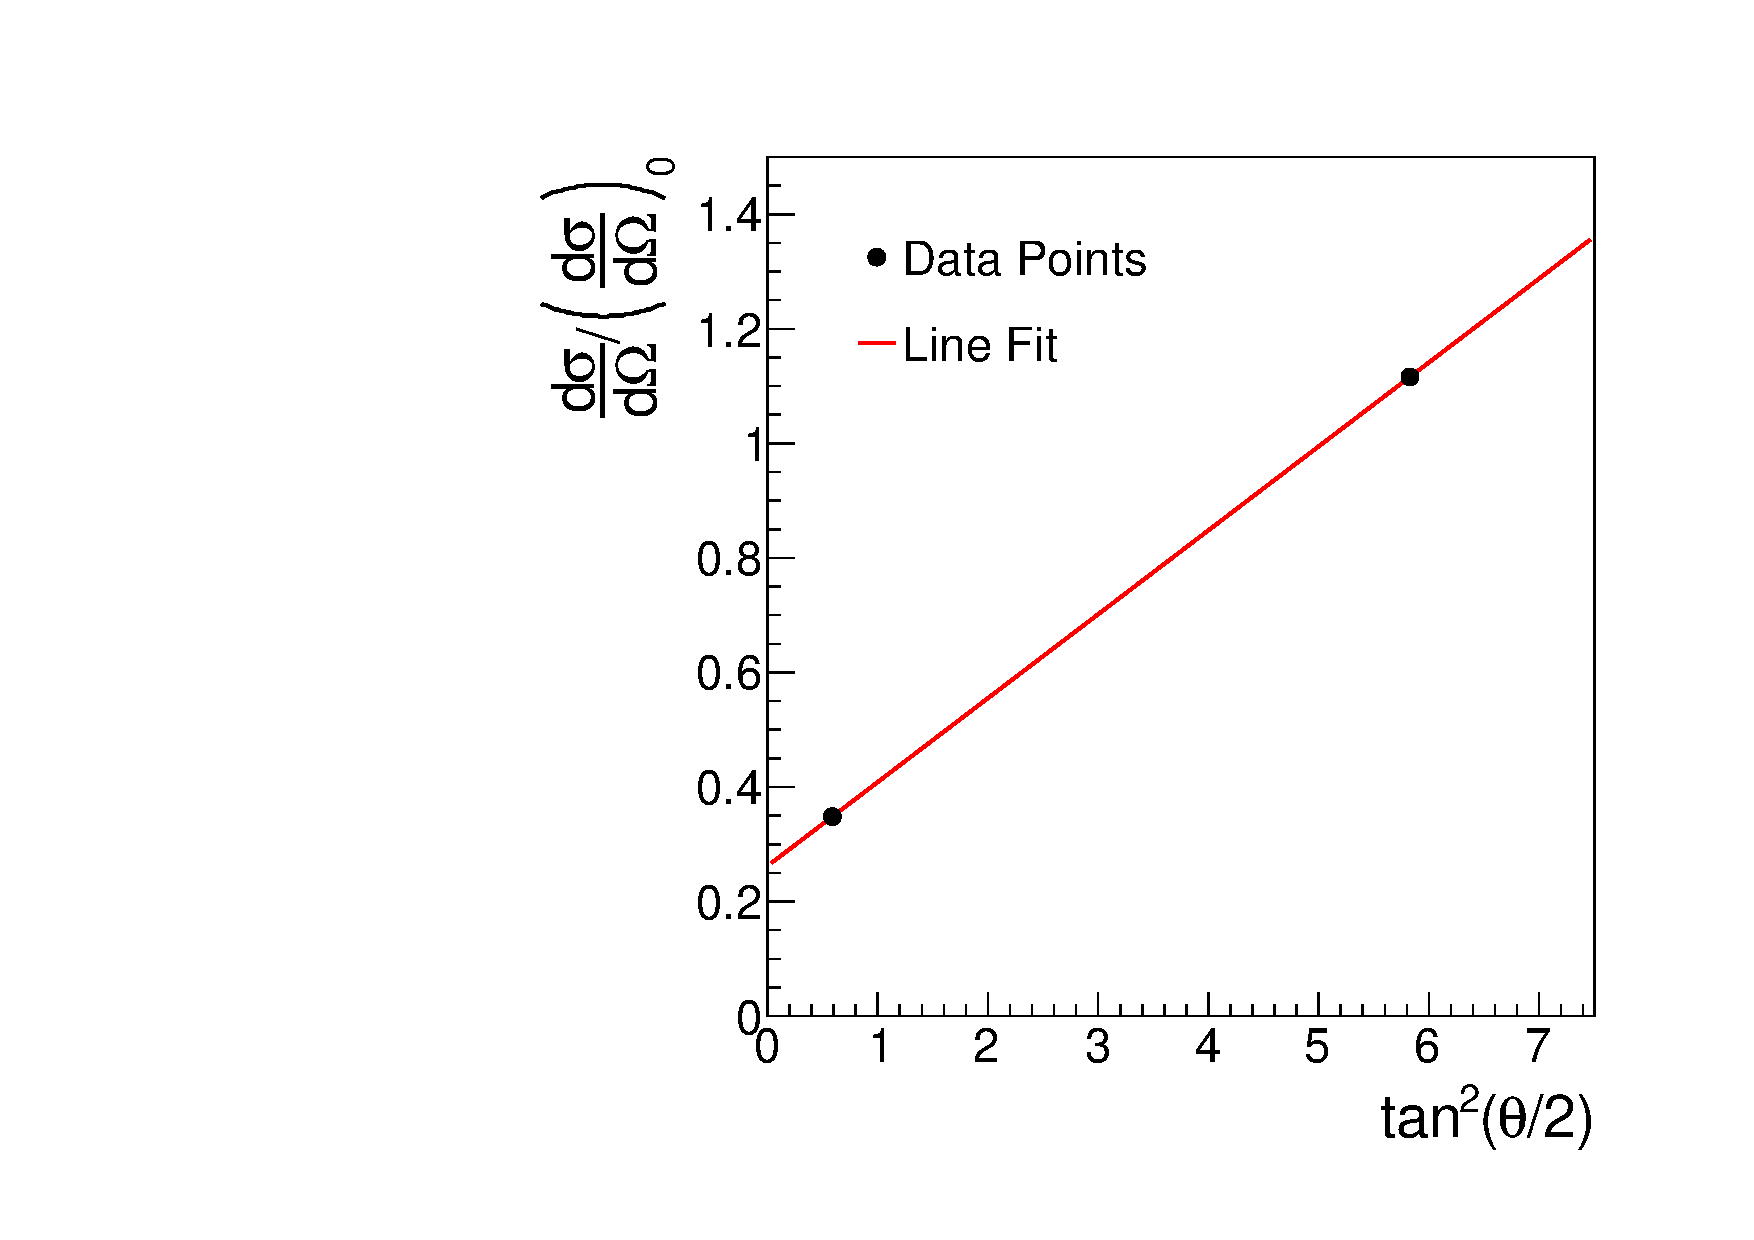
\includegraphics[width=0.575\textwidth]{Figures/Ch7/P7.7.pdf}
    \caption{Linear relation obtained for $Q^2=0.5\GeV^2$}
    \label{fig:P7.7}  
\end{figure}
  
The slope and intercept will be used to compute $G_M(Q^2)$ and $G_E(Q^2)$, where $\tau=Q^2/4m_p^2 \simeq 0.071$ :

\begin{align*}
    m \simeq 0.1465 = 2\tau \left[G_M(Q^2)\right]^2 \implies G_M(Q^2) \simeq \sqrt{\frac{0.1465}{2\cdot 0.071}}\simeq 1.015
\end{align*}\\

and using the intercept which is $\simeq 0.4$ one could get

\begin{align*}
    c \simeq 0.2620 = \frac{1}{1+\tau}\cdot \left[ G_E(Q^2)^2 + \tau G_M(Q^2)^2 \right] \implies G_E(Q^2)^2 \simeq  0.2620(1+0.071)-0.071 \cdot G_M(Q^2)^2 \simeq 0.2074
\end{align*}\\
Thus one could finally say that,

\begin{align*}
    G_E(0.5\GeV^2) \simeq \boxed{0.4554}
\end{align*}
\end{solution}

\noindent\rule{7in}{1.5pt}
 
%%%%%%%%%%%%%%%%%%%%%%%%%%%%%%%%%%%%%%%%%%%%%%%%%%%%%%%%%%%%%%%%%%%%%%%%%%%%%%%%%%%%%%%%%%%%%%%%%%%%%%%%%%%%%%%%%%%%%%%%%%%%%%%%%%%%%%%%

\begin{problem}{7.8}
    The experimental data of Figure 7.8 can be described by the form factor

    \begin{align*}
        G(Q^2)= \frac{G(0)}{\left( 1+Q^2/Q_0^2 \right)^2}
    \end{align*}\\
    with $Q_0^2 = 0.71 \GeV^2$. Taking $Q_2 \approx \mathbf{q}^2$, show that this implies that proton has an exponential charge distri-bution of the form

    \begin{align*}
        \rho(\mathbf{r}) = \rho_0 e^{-\frac{r}{a}}
    \end{align*}\\
    and find the value of a.
\end{problem}
\begin{solution}

\end{solution}

\noindent\rule{7in}{1.5pt}

%%%%%%%%%%%%%%%%%%%%%%%%%%%%%%%%%%%%%%%%%%%%%%%%%%%%%%%%%%%%%%%%%%%%%%%%%%%%%%%%%%%%%%%%%%%%%%%%%%%%%%%%%%%%%%%%%%%%%%%%%%%%%%%%%%%%%%%%
